\documentclass{article}

\usepackage{subfigure}
\usepackage{amssymb, amsmath, amsfonts}
\usepackage{amsthm}
\usepackage{tikz}
\usetikzlibrary{external}
\usepackage{pgfplots}

\newtheorem{proposition}{Proposition}
\newtheorem{theorem}{Theorem}
\newtheorem{definition}{Definition}
\newtheorem{lemma}{Lemma}
\newtheorem{conjecture}{Conjecture}
\newtheorem{corollary}{Corollary}
\newtheorem{remark}{Remark}
\newtheorem{assumption}{Assumption}

\newlength\figureheight
\newlength\figurewidth

\ifnum\pdfshellescape=1
\tikzexternalize[prefix=tikzpdf/]
\fi

\newcommand{\tikzdir}[1]{tikz/#1.tikz}
\newcommand{\inputtikz}[1]{\tikzsetnextfilename{#1}\input{\tikzdir{#1}}}

\DeclareMathOperator*{\argmin}{arg\; min}     % argmin
\DeclareMathOperator*{\argmax}{arg\; max}     % argmax
\DeclareMathOperator*{\tr}{tr}     % trace
\DeclareMathOperator{\Cov}{Cov}
\DeclareMathOperator{\logdet}{log\;det}

\title{Gossip Algorithm}

\author{Yilin Mo}

\begin{document} \maketitle

We model a network composed of $n$ agents as a graph $G = \{V,\,E\}$. $V = \{1,2,\ldots,n\}$ is the set of vertices representing the agents. $E \subseteq V\times V$ is the set of edges. $(i,j)\in E$ if and only if sensor $i$ and $j$ can communicate directly with each other. We will always assume that $G$ is undirected, i.e. $(i,j)\in E$ if and only if $(j,i)\in E$. We further assume that there is no self loop, i.e., $(i,i)\notin E$.

At each time step, we assume a pair of nodes $(i,j)$ is randomly selected with probability $p_{ij}$, where $(i,j)\in E$. They communicate with each other and perform the following update:
\begin{displaymath}
 x_i(k+1) = x_j(k+1) = (x_i(k)+x_j(k))/2 .
\end{displaymath}
All the other nodes that are not selected keep their own states:
\begin{displaymath}
  x_l(k+1) = x_l(k),\,\forall l\notin \{i,j\}.
\end{displaymath}

Let us define matrix
\begin{displaymath}
  W_{ij} = I - (e_i - e_j)(e_i-e_j)^T/2.
\end{displaymath}
Then the update equation can be written in matrix form as
\begin{displaymath}
  x(k+1) = W(k)x(k) = W_{ij} x(k) ,\text{ with probability }p_{ij}. 
\end{displaymath}

Define $y(k) = x(k) - x_{ave} = (I-J)x(k)$ (why?). 
\begin{displaymath}
 y(k+1) =   (W(k)-J) y(k).
\end{displaymath}

Problem:
\begin{itemize}
  \item Under what condition does $x(k)$ converges to the $x_{ave} = J x(0)$, where $J = \mathbf 1\mathbf 1^T/n$? 
  \item How fast is the convergence rate?
\end{itemize}
\section{Products of Random Numbers}

Let us assume that $\alpha(k)$ are i.i.d. distributed and define
\begin{displaymath}
 \beta(k) = \alpha(k)\dots\alpha(0). 
\end{displaymath}

\begin{enumerate}
  \item $\beta(k)$ converges to $0$ almost surely if
    \begin{displaymath}
      P(\lim_{k\rightarrow\infty}\beta(k) = 0) =1 .
    \end{displaymath}
  \item $\beta(k)$ converges to $0$ in $L_p$ if
    \begin{displaymath}
      \lim_{k\rightarrow\infty}  \mathbb E\beta(k)^p = 0.
    \end{displaymath}
    The $L_p$ convergence rate can be defined as
    \begin{displaymath}
      \rho_p=\sqrt[k]{\mathbb E\left(\beta(k)^p\right)}
    \end{displaymath}
    A special case is convergence in mean square sense:
    \begin{displaymath}
      \lim_{k\rightarrow\infty} \mathbb E\beta(k)^2 = 0 
    \end{displaymath}
\end{enumerate}

\begin{theorem}
  $\beta(k)$ converges in $L_p$ if and only if 
  \begin{displaymath}
   \rho_p = \mathbb E\left(\alpha(0)^p\right) < 1.
  \end{displaymath}
  Furthermore, 
  \begin{displaymath}
    P\left( \lim_{k\rightarrow\infty} \sqrt[k]{\beta(k)} = \exp\left[\mathbb E\left( \log\alpha(k)\right)\right] \right)=1. 
  \end{displaymath}
\end{theorem}
\begin{proof}
  Since $\alpha(k)$ are independent of each other,
  \begin{displaymath}
    \mathbb E\beta(k)^p = \prod_{t=0}^k \mathbb E\alpha(t)^p. 
  \end{displaymath}
  Hence, $\rho_p = \mathbb E\alpha(t)^p$.

  On the other hand,
  \begin{displaymath}
    \log \beta(k) = \sum_{t=0}^k \log \alpha(t). 
  \end{displaymath}
  By LLN,
  \begin{displaymath}
    \lim_{k\rightarrow\infty}\frac{\log \beta(k)}{k } = \mathbb E\left( \log \alpha(t) \right),\text{ almost surely}
  \end{displaymath}
\end{proof}
Let us assume that
\begin{displaymath}
  \alpha(k) = \begin{cases}
    0&\text{with probability }0.5\\
    2&\text{with probability }0.5
  \end{cases}
\end{displaymath}
Then $\beta(k)$ converges almost surely, but does not converge in $L_p$.

\section{Products of Random Matrices}
The following theorem can be seen as a generalization of LLN for noncommutative case
\begin{theorem}
  Let $X(k)$ be i.i.d. distributed, if
  \begin{displaymath}
   \mathbb E \left[\max(\log\|X(k)\|,0) \right]<\infty,
  \end{displaymath}
  then
  \begin{displaymath}
    \lim_{k\rightarrow\infty} k^{-1}\log\|X(k)X(k-1)\dots X(1)\| = \rho_{as},
  \end{displaymath}
  with probability 1, where $\rho_{as}$ is defined as
  \begin{displaymath}
    \rho_{as} =  \lim_{k\rightarrow\infty} k^{-1}\mathbb E\left(\log\|X(k)X(k-1)\dots X(1)\|\right).
  \end{displaymath}
\end{theorem}

For general cases, the almost surely convergence rate $\rho_{as}$ is still unknown.

Now let us consider the mean square convergence rate. First look at the $W_{ij}$ matrix, we know that
\begin{itemize}
  \item $W_{ij}$ is symmetric.
  \item $W_{ij}\leq I$. 
  \item $W_{ij}\mathbf 1 = \mathbf 1$.
\end{itemize}

Define 
\begin{displaymath}
  W \triangleq \mathbb E W(k) = \sum_{(i,j)\in E} p_{ij}W_{ij}.
\end{displaymath}

Therefore,
\begin{itemize}
  \item $W$ is symmetric.
  \item $W\leq I$. 
  \item $W\mathbf 1 = \mathbf 1$.
\end{itemize}

Define $\mathcal W = W-J$, then
\begin{displaymath}
 y(k+1) =   (W(k)-J) y(k)\implies \mathbb E y(k+1) = \mathcal W \mathbb E y(k).
\end{displaymath}
Therefore,
\begin{displaymath}
\mathbb E y(k)  = \mathcal W^k y(0).
\end{displaymath}

By Jensen's inequality,
\begin{equation}
\mathbb E \|y(k)\|^2\geq  \|\mathbb E y(k)\|^2   = \|\mathcal W^k y(0)\|^2.
\label{eq:lowerbound}
\end{equation}
Thus, there exists an $y(0)$ (which is the eigenvector of $\lambda_2(W)$, such that
\begin{displaymath}
  \mathbb E\|y(k)\|^2\geq \lambda_2(W)^{2k}\|y(0)\|^2 
\end{displaymath}


On the other hand,
\begin{displaymath}
 y(k+1)^Ty(k+1) = y(k)^T(W(k)-J)^2 y(k) = y(k)^T (W(k)-J) y(k).
\end{displaymath}
Hence,
\begin{displaymath}
 \mathbb E\| y(k+1)\|^2 =  \mathbb E\left[  y(k)^T \mathbb E((W(k)-J)|y(k)) y(k)\right] = \mathbb E\left[ y(k)^T\mathcal Wy(k) \right]\leq \lambda_2(W) \mathbb E\|y(k)\|^2.
\end{displaymath}
Thus,
\begin{displaymath}
 \mathbb E\|y(k)\|^2\leq \lambda_2(W)^k \|y(0)\|^2. 
\end{displaymath}

Hence, the mean square convergence rate satisfies
\begin{displaymath}
 \lambda_2(W)^2 \leq \rho_2 \leq \lambda_2(W).
\end{displaymath}

The gossip algorithm converges in the mean square sense if and only if $\lambda_2(W)<1$.

To get the exact mean square convergence rate, we need to consider
\begin{displaymath}
 Y(k) = y(k)y(k)^T. 
\end{displaymath}
Clearly,
\begin{displaymath}
 Y(k+1) = (W(k)-J)Y(k) (W(k)-J).
\end{displaymath}
Hence,
\begin{displaymath}
  \mathbb E Y(k+1) = \sum_{(i,j)\in E} p_{ij} (W_{ij}-J)\mathbb EY(k) (W_{ij}-J).
\end{displaymath}
If we define the operator $\mathcal A:\mathbb S_n\rightarrow\mathbb S_n$:
\begin{displaymath}
  \mathcal A(X) = \sum_{(i,j)\in E} p_{ij}  (W_{ij}-J)X (W_{ij}-J).
\end{displaymath}
$\mathcal A(X)$ is a linear operator on $\mathbb S_n$. The mean square convergence rate $\rho_2$ will be the operator norm of $\mathcal A$.

Examples:
\begin{figure}[h]
  \begin{center}
    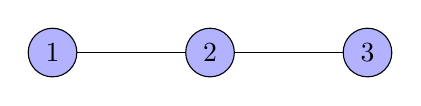
\begin{tikzpicture}
      \node [circle, draw, fill=blue!30] (1) at (0,0) {$1$};
      \node [circle, draw, fill=blue!30] (2) at (2,0) {$2$};
      \node [circle, draw, fill=blue!30] (3) at (4,0) {$3$};
      \draw [semithick] (1) to (2);
      \draw [semithick] (2) to (3);
    \end{tikzpicture}
  \end{center}
\end{figure}

Assume that $p_{12} = 0.5$, $p_{23} = 0.5$. Hence,
\begin{displaymath}
  W = \frac{1}{4}\begin{bmatrix}
    3&1&0\\
    1&2&1\\
    0&1&3
  \end{bmatrix}.
\end{displaymath}
The eigenvalues are $1, 0.75, 0.25$. The corresponding eigenvectors are
\begin{displaymath}
  v_1 = \begin{bmatrix}
    1\\
    1\\
    1\\
  \end{bmatrix}, v_2 = \begin{bmatrix}
    1\\
    0\\
    -1\\
  \end{bmatrix}, v_3 = \begin{bmatrix}
    -1\\
    2\\
    -1\\
  \end{bmatrix}.
\end{displaymath}
Hence, we know that $9/16\leq \rho_2 \leq 3/4$. Now let us define
\begin{displaymath}
    v_a = \begin{bmatrix}
    1\\
    1\\
    -2\\
  \end{bmatrix}, v_b = \begin{bmatrix}
    -2\\
    1\\
    1\\
  \end{bmatrix}
\end{displaymath}
We argue that $y(k)$ is either $\theta(k) v_a$ or $\theta(k) v_b$. (Why?)

If $y(k) = \theta(k) v_a$, then if $(1,2)$ is selected, $y(k+1) = y(k)$. On the other hand, if $(2,3)$ is selection, then
\begin{displaymath}
  y(k+1) = \theta(k)\begin{bmatrix}
1\\
-0.5\\
-0.5\\
  \end{bmatrix} = -\frac{\theta(k)}{2}v_b.
\end{displaymath}
Hence
\begin{displaymath}
  \|y(k+1)\|^2 = \begin{cases}
    \|y(k)\|^2&\text{ with probability }0.5\\
    0.25\|y(k)\|^2&\text{ with probability }0.5
  \end{cases}
\end{displaymath}
The true mean square convergence rate should be
\begin{displaymath}
  \rho_2 = 0.5\times 1 + 0.5\times 0.25 = \frac{5}{8}.  
\end{displaymath}
\end{document}



